%\documentclass[12pt,a4paper]{article}
\documentclass[12pt]{article}
\usepackage[utf8x]{inputenc}
\usepackage{ucs}
\usepackage{amsmath}
\usepackage{verbatim} 
\usepackage{amsfonts}
\usepackage{amssymb}

\author{
	Llu\'{i}s-Pere de las Heras Caballero \and
	Ahmed Mounir Gad \and
	Monica Pi\~{n}ol 
}


\title{Face recognition and tracking}

\begin{document}

\maketitle
\thispagestyle{empty}
\newpage

\section{Introduction}
In this project our main focus is to build a single and multiple target tracker. We extend this approach to build a useful reallife application to that tracker which is a face recognizer and tracker.

Our project first starts the normal tracking process which is segmentation and only determining the useful parts of the scene. We use these useful parts of the scene to detect the faces and correspond these faces to the interesting faces in the scene. We afterwards calculate the velocity of the person having this face and we keep tracking until the person leaves the scene or our tracker fails.
\section{Segmentation}
The process of segmentation is to separate the background to foreground.

\begin{itemize}
\item The Background subtraction use three parameters: \textbf{gamma},\textbf{tau} and \textbf{radius}.
	$ Background_{i+1} = gamma*frame_{i} + (1-gamma)*Background_{i}$
	\begin{itemize}
	\item Gamma is the learning rate, usually is 0,05.
	\item Tau is the different between frame to background.
	\item Radius is the parameter to delete the little blobs.
	\end{itemize}
	
\item The \textit{background subtraction} is not robustness to change illumination, for this we implement \textit{Grey-World} because is invariant to illuminant changes. 
The Grey-World method try to eliminate the gray in the image, for this reason move the minimum and the maximum values.

\begin{equation}
	( R' G' B' )= \left(
	\begin{array}{ccc}
		\frac{R_{grey}}{R_{m}(I)}  0  0 \\
		0  \frac{G_{grey}}{G_{m}(I)}  0 \\
 		0  0  \frac{B_{grey}}{B_{m}(I)}
	\end{array}
	\right) 
	* 
	\left(
	\begin{array}{c} R \\ G \\ B
	\end{array}
	\right)
\end{equation} 

\item Selectivity is the other method that use the simple different between foreground with background but the selectivity a prior knows that pixel is or isn't foreground. 

\item Eigenbackground
\end{itemize}
 
\section{Detection}

Up to here, the \textbf{Segmenter} has finished its work and we have a number of blobs that correspond to the changes in the background. Some of these changes are definitely the objects we are interested in. This step in the tracker mainly focuses on detecting the important parts of these background changes.

The basic detector provided in our framework is based on simple blob detection. It just returns each set of connected pixels as an object. We basically have two questions to investigate about. The first is how the basic tracker provided behave in the presence of noisy detection. The second is how the tracker behaves in the case of no detection. The answers to these two questions are illustrated in the tracking section.

We did several optimizations to the simple detector provided. The first was to detect faces and keep tracking those detected faces. It was used the Viola and Jones AdaBoost Face-Detector[2]. We thought of an interesting application that may use this technique. We added a face recognizer that only detects faces of people of interest to the tracker. We provide a trained Support Vector Machine(SVM) classifier to our tracker. We train it using labeled faces detected from a video for 5 persons. In total 364 faces for 5 people were used for training and all taken from one single video. The \textbf{Detector} then will only detect the people of interest in any video and the tracker will only track those people.

\begin{figure}[Face detection and recognition]{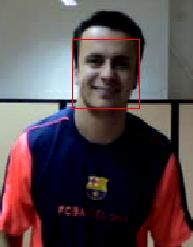
\includegraphics[width=0.3\textwidth]{det_lluis}}
  \centering
  \caption{Face detected and recognized as Lluis}
\end{figure}

In case a match was found, the \textbf{Detector} will return the bounding box of the face that made that match. We thought as an improvement we may try to detect the whole body of the person who made that match. However, plenty of noise coming from the background made this process hard and time consuming. We stopped at this step only satisfied with detecting the face's bounding box and passing it to the \textbf{Representer}.

On the other hand, the \textbf{Detector} may not be able to detect and recognize any face in a certain frame. In this case, the \textbf{Detector} return all those blobs that their \textit{bounding-box} is larger than appropriate threshold. This is done to delete too small noisy blobs and just being interested in those ones that could be a person. The representer will be the responsible to assure if these blobs are belonging to people who was tracked in the last frame.
\section{Representation}
\section{Tracking}

In this section we will discuss the main module of the project which is the tracker. A simple Kalman filter tracker has been provided in the tracking framework. It uses results of the representer to track the position and the extent of the object being tracked. The Kalman filter works by estimating an unobservable state which is updated in time with a linear state update and additive Gaussian noise. It uses the technique described in \cite{Arulampalam01atutorial}.

%%%%%%%%%%%%%%%%%%%%%%%%%%%%%%%%%%%
%%                                                                                                                  %%
%%   Here we should answer the two provided questions.                            %%
%%   We should also solve the problems proposed in the detection part.     %%
%%                                                                                                                  %%
%%%%%%%%%%%%%%%%%%%%%%%%%%%%%%%%%%%


\section{Conclusion}

\bibliographystyle{plain}
\bibliography{bibfile}

\end{document}
